\documentclass[aspectratio=169]{beamer}
%\documentclass[handout]{beamer}

% language settings
%\usepackage{fontspec, polyglossia}
%\setdefaultlanguage{magyar}

% common packages
\usepackage{amsmath, multimedia, hyperref, color, multirow}
%\usepackage{graphicx}
\usepackage{pifont}

% TikZ
\usepackage{tikz}
\usetikzlibrary{arrows.meta, decorations.pathmorphing, decorations.pathreplacing, shapes.geometric,mindmap}
\usetikzlibrary{shapes.geometric,fadings,bayesnet}

% beamer styles
\mode<presentation>{
\usetheme{Pittsburgh}
%\usetheme{Antibes}
\usecolortheme{beaver}
%\usecolortheme{seahorse}
%\usefonttheme{structureitalicserif}
\setbeamercovered{transparent}
}
\setbeamertemplate{blocks}[rounded][shadow=true]
\AtBeginSubsection[]{
  \begin{frame}<beamer>{Contents}
  \end{frame}
}
%\useoutertheme[]{tree}

% title, etc
%\title{Drug Repurposing to Alzheimer's Disease Using TWAS and the PPI Network}
\title{Alzheimer's Disease Genes}
\author{Attila Jones}
\date{National Institute of Health}

\begin{document}

\maketitle

\section{Introduction}

\begin{frame}{Alzheimer's disease}
\begin{columns}[t]
\begin{column}{0.5\textwidth}
Implicated processes
\begin{itemize}
\item lipid, sugar metabolism
\item immune function
\item synaptic function
\end{itemize}

Relevant cell types, tissues
\begin{itemize}
\item brain: microglia, neurons
\item blood
\item ...?
\end{itemize}
\end{column}

\begin{column}{0.5\textwidth}
Genetics
\begin{itemize}
\item 26 genes in knowledge bases
\item 37 GWAS loci
\item fine mapping, gene prioritization studies
\end{itemize}


\end{column}
\end{columns}
\end{frame}

\begin{frame}{Drug repurposing}
\begin{columns}[t]
\begin{column}{0.6\textwidth}

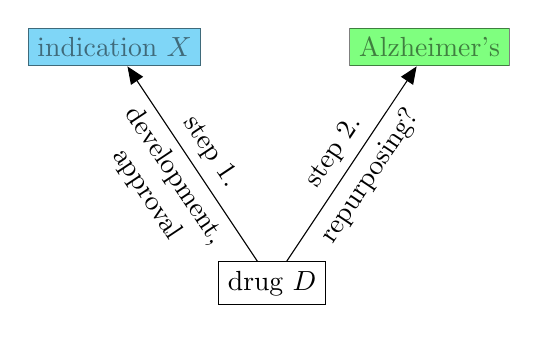
\begin{tikzpicture}
\path (0,0) node[draw] (drug) {drug $D$}
	(-2,3) node[draw,fill=cyan,semitransparent] (ind) {indication $X$}
	( 2,3) node[draw,fill=green,semitransparent] (alz) {Alzheimer's};
\path[->] (drug) edge node[below,sloped,text width=3cm,text centered] {development, approval} node[above,sloped]
	{step 1.} (ind);
\path[->] (drug) edge node[below,sloped] {repurposing?} node[above,sloped]
	{step 2.} (alz);
\end{tikzpicture}
\end{column}

\begin{column}{0.4\textwidth}
Approaches to repurposing
\begin{enumerate}
\item shared gene approach\\
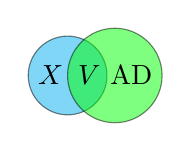
\begin{tikzpicture}
\draw[fill=cyan,semitransparent] (0,0) circle (0.5cm);
\draw[fill=green,semitransparent] (0.6,0) circle (0.6cm);
\draw (0.275cm,0) node {$V$};
\draw (1.2cm,0) node[anchor=east] {AD};
%\draw (0.6cm,0.6) node[anchor=south] {AD};
\draw (-0.5cm,0.0) node[anchor=west] {$X$};
\end{tikzpicture}

\tiny
overlap $V = X \cap \mathrm{AD}$
\normalsize
\item network based appr.
\begin{description}
	\tiny
\item[Guney,..., Barabási 2016] proximity
\item[Cheng,..., Barabási 2018] validation
\end{description}
\end{enumerate}
\end{column}
\end{columns}
\begin{center}
	\Large \alert{AD gene set $= \overbrace{\{\mathrm{APOE}, \mathrm{APP},
		...\}}^{\text{knowledge (26 genes)}} +
	\overbrace{\{?,?,...\}}^{\text{omics}}$}
\end{center}
\end{frame}

\begin{frame}{GWAS: fine mapping, gene prioritization}
\begin{columns}[t]
\begin{column}{0.4\textwidth}
\begin{itemize}
\item TWAS
\begin{itemize}
\item MR or PrediXcan
\item colocalization
\end{itemize}
\item PWAS
\item GWGAS
\item 3D chromatin,...
\end{itemize}
\end{column}

\begin{column}{0.7\textwidth}

\includegraphics[width=\columnwidth]{figures/from-others/jian-yang-2016-fig1.png}

{\tiny Zhu et al 2016 Nat Genet}
\end{column}
\end{columns}
\end{frame}

\begin{frame}{Summary of published TWAS experiments}{See Google sheet}
\begin{enumerate}
\item Credibility of each experiment?
\begin{itemize}
	\item design, methods
	\item tissue relevance
	\item sample size
\end{itemize}
\item Concordance among experiments?
\item Is it worth to carry out our own experiment?  If yes, how?
\end{enumerate}
\end{frame}

\begin{frame}{Discordance of TWAS (or PWAS) experiments}
\includegraphics[scale=0.45]{../../../notebooks/2021-07-01-high-conf-ADgenes/named-figure/no-experiments-inferring-the-same-gene.pdf}
\includegraphics[scale=0.45]{../../../notebooks/2021-07-01-high-conf-ADgenes/named-figure/cluster-experiments-genes.pdf}
\end{frame}

\begin{frame}{TWAS (or PWAS) confirms few known AD genes}
	{Take genes supported by multiple TWAS experiments?}
\begin{columns}[t]
\begin{column}{0.35\textwidth}

\includegraphics[width=\columnwidth]{../../../notebooks/2021-07-01-high-conf-ADgenes/named-figure/knowledge-twas-proteo-venn.pdf}
\end{column}
\begin{column}{0.35\textwidth}

\includegraphics[width=\columnwidth]{../../../notebooks/2021-07-01-high-conf-ADgenes/named-figure/knowledge-twas-2plus-proteo-venn.pdf}
\end{column}

\begin{column}{0.35\textwidth}

\includegraphics[width=\columnwidth]{../../../notebooks/2021-07-01-high-conf-ADgenes/named-figure/knowledge-twas-3plus-proteo-venn.pdf}
\end{column}
\end{columns}
\end{frame}

\end{document}


\begin{columns}[t]
\begin{column}{0.5\textwidth}

\end{column}

\begin{column}{0.5\textwidth}

\end{column}
\end{columns}
